\documentclass[a4paper,11pt]{report}

\usepackage[english, polish]{babel}
\usepackage[utf8]{inputenc}
\usepackage{blindtext}
\usepackage[T1]{fontenc}
\usepackage{booktabs}
\usepackage{graphicx}
\usepackage{wrapfig}
\usepackage{multirow}
\usepackage[export]{adjustbox}
\usepackage[nottoc,notlot,notlof]{tocbibind}

\begin{document}
\let\cleardoublepage\clearpage
\begin{figure}[ht]
\centering

\includegraphics{pjatk.png}
\end{figure}
\begin{center}
\textbf{\huge Karta Projektu}\\
\vspace{1cm}
\begin{tabular}{|p{15cm}|}
\hline
\textbf{Temat projektu:}\\Gamitude manage your Energy, not your Time\\ 
\hline
\textbf{Akronim:}\\GTM\\
\hline
\textbf{Opiekun:}\\Tadeusz Puźniakowski  \\
\hline
\textbf{Konsultanci:}\\Tadeusz Puźniakowski\\Marek Bednarczyk \\
\hline
\textbf{Cele projektu:}
\\Dostarczenie użytkownikom narzędzia do zarządzania ich energią,
 opartego o najnowsze odkrycia dotyczące ludzkiej produktywności.
Jednocześnie chcemy,
 aby użytkownicy zaczęli postrzegać prace bądź naukę bardziej pozytywnie dzięki powiązaniom pracy z elementami gier RPG.\\
\hline
\textbf{Rezultaty projektu:}\\Kompletny system do zarządzania projektami opierający się na najnowszych badaniach dotyczących ludzkiej produktywności. \\
\hline
\textbf{Miary sukcesu:}\\Działający system projektów, Bullet Journal, Gamitude Themes.\\
\hline
\textbf{Ograniczenia:}\\Czasowe, umiejętnościowe, budżetowe \\
\hline
\end{tabular}\\
\vspace{1cm}
\begin{tabular}{|l|l|l|l|}
\hline
\textbf{Wykonawca} & \textbf{Numer albumu}& \textbf{Specjalizacja}& \textbf{Tryb studiów} \\
\hline
Robert Deyk&s17707&SI&Stacjonarne \\
\hline
Paweł Benkowski&s16569&SI&Stacjonarne\\
\hline
Stanisław Lutkiewicz&s17535&SI&Stacjonarne \\
\hline
\end{tabular}\\
\vspace{1cm}
\begin{tabular}{|l|l|l|l|}
\hline
\textbf{Data ukończenia projektu:} & to be determined & \textbf{Recenzent:} & to be determined\\
\hline
\end{tabular}
\end{center}
\tableofcontents

\chapter{Wprowadzenie}
\section{Kontekst pracy}
Energie\cite{Harward} dzielą się na 4 rodzaje: duszy, ciała, emocji i umysłu.
\\Istnieją różne techniki próbujące wspomóc ich efektywne wykorzystywanie jak metoda Pomodoro\cite{Pomodoro} czy Ultradian Rhythm\cite{90/30}.
\\\\Pierwsza technika polega na dzieleniu czasu pracy na 25-minutowe sesje, po których następuje 5-minutowa przerwa.
 Po wykonaniu 5 takich sesji przerwa wydłuża się do 15 minut.
 Technika ta jest szczególnie przydatna podczas nauki.
\\Jak wiadomo z badań, po nauce należy dać mózgowi czas na 'przetworzenie' nowych informacji.
 Tworzy on w tym czasie nowe synapsy, dołączając nowo nabytą wiedze do istniejącej sieci informacji.
 Jeżeli napotka terminy podobne do nowej informacji, połączy je,  umacniając strukturę. 
\\\\Druga technika polega na dzieleniu czasu na pracy na 90-minutowe sesje, po których następuje 30-minutowa przerwa.
 Technika ta jest oparta na naturalnym cyklu ludzkiej aktywności podczas dnia.
 Ultradian Rhythm jest szczególnie przydatny przy zadaniach rutynowych bądź częściowo rutynowych.
 Przykładem takiego zadania jest praca.
\\\\Są to tylko dwie najpopularniejsze metodyki pracy, dzięki którym zwiększamy swoją wydajność,
 ale wciąż prowadzimy badania nad tym tematem, szukając nowych technik,
 tak aby Gamitude oferował, jak najszersze możliwości personalizacji. 
\\\\Niekiedy jednak projekty trzeba rozplanować jako zadania w kontekście czasu.
 Na takie okazje planujemy stworzyć Bullet Journal\cite{bullet}'a.
 Jest to dziennik ze stronami dedykowanymi na zadania z terminem na dzisiaj,
  na za tydzień, na za miesiąc bądź w nieokreślonej przyszłości.
\\\\Aby użytkownik czuł, że jego praca przynosi efekty dodamy również elementy grywalizacji\cite{grywalizacja}, czyli 
 statystyki oraz rangi\cite{rangi}, gdzie statystyki można rozumieć jako sztuczną walutę podzieloną na 4 rodzaje a rangi 
 jako awatara użytkownika kupowanego za te waluty.
\section{Przedstawienie problemu}
Według pracy harwardzkiej, ludzie organizujący sobie prace, mają tendencje do siadania i wykonywania jej bez przerwy aż do ukończenia,
 ignorując holistyczną naturę działania ludzkiego organizmu oraz naturalne cykle zachodzące w ludzkim ciele.
 W pracy czas jest porównywany do węgla a energia do wiatru.
 Jest to nawiązanie do przemysłu energetycznego i cech źródeł odnawialnych i nieodnawialnych.

\section{Cel i zakres projektu}
Celem jest stworzenie systemu, który swoje działanie bazuje na energiach omówionych wcześniej,
 zwracając także uwagę na nie przepracowywanie użytkowników.
\vspace{0,5cm}
Zakresem projektu jest stworzenie zestawu narzędzi szanujących higienę pracy
 oraz indywidualne preferencje organizacji pracy przez użytkowników.

\section{Podejście do projektu}
Zwinne, Scrumban, aplikacja webowa oparta o JS, backend w .NET, wybrane ze względu na wieloplatformowość.

\section{Rezultaty}
Ludzie potrafią utrzymać produktywność w dłuższym okresie, bez ubytków w żadnej z dziedzin życia.

\section{Organizacja dokumentu}
Omówienie problemu, analiza projektu, projektowanie i implementacja systemu, historia implementacji,
 testy systemu, testy w grupie docelowej, nakład pracy, wkład własny, podsumowanie

\section {Słownik pojęć}
	\emph{Bullet Journal – dziennik, w którym można rozplanowywać zadania}\\
	\emph{Elastic Habits – stopniowanie zadania na 3 poziomy}\\
	\emph{Projekt – Czynność bądź umiejętność, nad którą użytkownik chce pracować, nie ma podziału na podpunkty, skupiający się na czasie}\\
	\emph{Statystyki-}\\
	\emph{Energie-}\\
	\emph{Rangi-}\\
	\emph{Motywy-}\\
	\emph{Tier-}\\
	\emph{Foldery-}\\
	\emph{Notatniki-}\\
	\emph{Strony-}\\
	\emph{Zadania-}\\
	\emph{Boosted statistics-}\\
	\emph{Dominant statistic-}\\
	\emph{Czasomierz-}\\
	

\chapter {Omówienie problemu}
\section {Przedstawienie problemu}
\subsubsection{Problem a ludzie}
Problemem jest bycie produktywnym.
\\Są ludzie, którzy nie robią absolutnie nic, dopóki nie są do tego przymuszeni.
\\Są tacy, którzy z każdym zadaniem czekają do ostatniej chwili, potem przepracowują się i powtarzają ten cykl.
\\Są też tacy, którzy starają się za bardzo i gdy w końcu ich organizm się buntuje, popadają w długie okresy nieróbstwa.
\\I na koniec są też pracoholicy, którzy tłumią zbuntowany organizm i dopiero choroba taka jak rak odciąga ich od pracy.
\\Wszystko to są objawy braku higieny pracy i nieefektywność w wykorzystywaniu energii.
\vspace{1cm}
\\Człowiek nierobiący nic zawsze ma jej pełno, chociaż wydaje mu się, że nie ma jej wcale.
\\Prokrastynator ma wrażenie, że energia pojawia się znikąd dopiero chwile przed terminem oddania.
\\Ci, którzy się starają, na początku każdego okresu nieróbstwa mają wrażenie, że po raz kolejny przegrali walkę z lenistwem.
\\Pracoholicy natomiast mają wrażenie, że są pełni energii, chociaż od dawna jadą na pustym baku.
\\Chociaż nie każdy popada w wymienione ekstrema, dobrze obrazują one ogólny problem z efektywnym wykorzystaniem energii.
\vspace{1cm}
\\Większość ludzkości nie utrzymuje stałego tempa pracy, na bieżąco wykonując wszystkie zaplanowane zadania.
\\Zamiast tego wahają się między stanami „Jestem do tyłu z robotą, trzeba się spieszyć” a „Jestem do przodu z robotą, mogę teraz tydzień nic nie robić”.
\subsubsection{Co i dlaczego nie działa?}
Ludzie operują w kontekście czasu i właśnie go próbują rozplanowywać. Jednakże czas jest surowcem skończonym, którego wszyscy ludzie mają dokładnie tyle samo.
\\Posiadając już te wiedze, ludzie wpadają w następną pułapkę hasłowego „nie liczy się to, ile masz czasu, ale jak go wykorzystasz”.
\\Jednak taki sposób myślenia jest typowy dla ludzi przepracowujących się, ponieważ czują, że czas im ucieka, i muszą za wszelką cenę nie dopuścić do zmarnowaniu choćby sekundy.
\\To pokazuje, jak chorobliwe jest skupienie myśli na czasie i zignorowanie lub błędna interpretacja sygnałów własnego organizmu.
\section {Rich picture}
\section {Konkurencyjne rozwiązania}
\subsection{Brain Focus}
\subsubsection{O Aplikacji}
Brain Focus jest to aplikacja mobilna, pozwalająca na odmierzanie czasu w sesjach z przerwami.
 Nie jest skomplikowana w użyciu, poprzez dosyć prosty wygląd co nie rozprasza użytkownika.
 Daje ona możliwość pełnej modyfikacji ich minutnika od czasu pracy i długości przerwy do ich ilości i częstości występowania dłużej przerwy.
 Posiada ona również funkcję blokowania innych aplikacji, by pomóc użytkownikom pozostać skupionym.
 Aplikacja również daje nam dostęp do ogólnych statystyk użytkownika tj. średnia długość pracy nad zadaniami itp.
\subsubsection{Zalety i wady}
Na pewno zaletami aplikacji jest jej prosty wygląd,
 jak i pełna możliwość modyfikacji minutnika,
 który może zostać przypisany do konkretnego zadania.
\vspace{0,5cm}
 \\Do jej wad można zaliczyć brak nagradzania użytkownika za jego poświęcony czas z aplikacją.
\vspace{0,5cm}
\\Chcielibyśmy wykorzystać ich zalety w formie pełnej modyfikacji minutnika razem z możliwością przypisywania go do zadania,
 ponieważ w naszym rozwiązaniu oczekujemy,
 że użytkownicy będą mieli bardzo zróżnicowane projekty, co spowoduję potrzebę modyfikacji minutnika pod projekty.
\subsubsection{Model biznesowy i popularność}
Aplikacja ta używa modelu biznesowego `freemium` gdzie w podstawowej formie aplikacja nie wysyła powiadomień
 oraz ma limitowane tworzenie kategorii zadań natomiast w wersji Pro
 po zakupieniu mamy nielimitowane tworzenie kategorii zadań,
 dostajemy dostęp do powiadomień w aplikacji,
 uzyskujemy dostęp do jej widget'u,
 jak i dostęp do wszystkich przyszłych funkcji aplikacji.
\vspace{0,5cm}\\Obecnie popularność aplikacji na platformie Google Play w liczbie pobrań przekracza 1000000 pobrań.
\subsection{Productivity Challenge Timer}
\subsubsection{O Aplikacji}
PCT jest to aplikacja mobilna, pozwalająca na dodawanie projektów,
 nad którymi chcemy pracować i umożliwia nam pracę nad nimi z odliczaniem czasu pracy w formie minutnika.
 Wraz z systematycznym pracowaniem nad naszymi projektami,
 aplikacja nagradza nas nowymi rangami w zależności od poświęconego czasu i systematyczności.
 Aplikacja prowadzi podstawowe statystyki tj. ilość sesji wykonana przy danym projekcie w danym dniu
 czy średnia ilość sesji w tygodniu. Jest także system osiągnięć, które zdobywamy wraz z używaniem aplikacji.
\subsubsection{Zalety i wady}
Zaletą aplikacji jest to, że aplikacja wynagradza użytkownika za spędzany z nią czas w formie rang,
 które ulepszają się wraz z systematyczną pracą.
\vspace{0,5cm}
\\Do jej wad możemy zaliczyć ograniczenie możliwości tworzenia projektów do 4 w darmowej wersji aplikacji,
ograniczona edycja minutnika, jak i duże kary za brak systematyczności w formie dużych spadków w rangach użytkownika.
System może również powodować przyśpieszone wypalenie, bądź nieefektywną prace poprzez zachęcanie do ciągłej, nieprzerwanej pracy.
\vspace{0,5cm}
\\Chcielibyśmy wykorzystać formę gratyfikacji użytkownika w formie rang, tak by nasza aplikacja
 jednocześnie motywowała naszych użytkowników do dalej pracy z systemem, jak i
 wykazywała postępy osiągane przez użytkownika.
\subsubsection{Model biznesowy i popularność}
Aplikacja używa modelu `freemium` gdzie w darmowej wersji jesteśmy ograniczeni do stworzenia 4 projektów,
 otrzymujemy agresywne reklamy w aplikacji, jak i mamy ograniczoną liczbę osiągnięć do zdobycia.
 Natomiast w wersji PRO mamy nieograniczoną liczbę projektów do tworzenia, nie dostajemy reklam,
 odblokowujemy dostęp do obecnie niemożliwych do zdobycia osiągnięć, jak i w przyszłości nowych.
\vspace{0,5cm}\\
Obecnie popularność aplikacji na platformie Google Play w liczbie pobrań przekracza 500000 pobrań.
\subsection{Habitica}
\subsubsection{O Aplikacji}
Habitica to aplikacja mobilna, jak i webowa, w której tworzymy swoją postać i ulepszamy ją poprzez wykonywanie zadań.
 Użytkownik na początku tworzy postać, którą rozwija wraz z używaniem aplikacji.
 Postać posiada statystyki tj. siła, inteligencja, kondycja i percepcja.
 Wraz z wykonywaniem zadań, postać zadaję określone punkty obrażeń stworą,
 które jeśli zostaną pokonane, dają postaci punkty doświadczenia.
 Punkty doświadczenia po osiągnięciu pewnego progu, zwiększają poziom postaci.
 Statystyki możemy zwiększać poprzez dodawanie ich za dostępne punkty po osiągnięciu poziomu bądź z posiadanych przedmiotów.
\subsubsection{Zalety i wady}
Zaletą aplikacji jest widoczna gamifikacja, co przyciąga dużą grupę użytkowników,
 która kojarzy owe systemy doświadczenia i statystyk z gier komputerowych.
 Zaletą również jest element aplikacji, gdzie tworzymy drużynę z innymi graczami, by pokonać silniejsze stwory.
\vspace{0,5cm}
\\Wadą aplikacji jest brak możliwości śledzenia czasu na wykonanie zadania bądź brak jakiegokolwiek minutnika, zachęcającego do systematycznej pracy.
 Wadą także jest duże skomplikowanie aplikacji, co może odstraszyć nowych użytkowników.
\vspace{0,5cm}\\
Chcielibyśmy wykorzystać system statystyk konta w naszym systemie,
 ponieważ idzie to w parze z osiąganiem rang jako forma nagradzania użytkownika za spędzany czas.
\subsubsection{Model biznesowy i popularność}
Model biznesowy aplikacji opiera się o mikro transakcje, gdzie możemy wykupywać walutę premium w grze,
 by osiągnąć rzeczy niedostępne dla użytkowników bez owej waluty tj. wyglądy postaci,
 misje na otrzymanie towarzyszy w formie chowańców czy możliwość zresetowania postaci.
\vspace{0,5cm}\\
Obecnie popularność aplikacji na platformie Google Play w liczbie pobrań przekracza 1000000 pobrań
 oraz szacowana ilość całkowita wszystkich użytkowników oscyluje w granicach 4000000 użytkowników.
\subsection{Pomodone}
\subsubsection{O Aplikacji}
Pomodone to aplikacja webowa, jak i mobilna, gdzie mamy możliwość dodawania zadań do wykonania
 oraz mamy możliwość włączenia sesji pracy nad konkretnym zadaniem.
 Aplikacja pozwala nam na zablokowanie konkretnych stron bądź aplikacji,
 by zapewnić użytkownikom pełne skupienie nad wykonanym zadaniem.
\subsubsection{Zalety i wady}
Zaletą aplikacji jest jej wieloplatformowość,
 ponieważ jest dostępna na każdym systemie operacyjnym, na komputerach stacjonarnych, systemach mobilnych,
 jak i przeglądarkach w formie widget'u.
 Kolejną zaletą jest też duża możliwość modyfikacji minutnika.
\vspace{0,5cm}
\\ Wadą jest pozornie prosty wygląd aplikacji, w której bardzo łatwo można się zgubić, będąc nowym użytkownikiem.
Wadą także można by nazwać brak podpowiedzi dla użytkownika, jeśli zgubiłby się w aplikacji.
\vspace{0,5cm}
\\Chcielibyśmy nie popełnić błędu, gdzie użytkownik bardzo łatwo może się zgubić w aplikacji,
 dlatego chcemy wytworzyć system, gdzie wszystkie potrzebne informacje zawsze będą na widoku
 oraz użytkownicy również będą mieli do dyspozycji podpowiedzi, jeśli mieliby trudności z korzystania z systemu.
\subsubsection{Model biznesowy i popularność}
Model biznesowy aplikacji używa płatnej subskrypcji do korzystania z aplikacji.
 Dla studentów jest rok darmowej subskrypcji dzięki programowi Github Education.
\vspace{0,5cm}\\
Obecnie popularność aplikacji na platformie Google Play w liczbie pobrań przekracza 10000 pobrań.
 Brak informacji o użytkownikach z innych platform.
\section {Propozycja rozwiązania}
Użytkownik będzie miał do wyboru kilka schematów organizacji pracy, każdy z nich będzie szanował ideę skupienia na energii zamiast na czasie.
\\Każda czynność będzie dodawała jedną, bądź kilka z 4 statystyk albo odnawiała jedną, bądź kilka z 4 energii.
\\Statystyki i odpowiadające energie:
\\Siła dla zadań fizycznych oraz odpowiadająca jej energia ciała.
\\Twórczość dla zadań artystycznych oraz odpowiadająca jej energia emocji.
\\Inteligencja dla zadań umysłowych oraz odpowiadająca jej energia umysłu.
\\Biegłość dla zadań humanistyczno-językowych oraz odpowiadające jej energia duszy.
\subsection{Projekty}
Pierwszym z nich są projekty, czyli organizacja ogólnej tematyki kierunku działań bądź konkretny plan bez wyszczególnionych celów pośrednich.
\\Użytkownik ma w tym wypadku jakiś cel, na tyle odległy, że wykonanie go nie jest możliwe podczas jednej, nieważne jak długiej, sesji pracy.
\\Przykładami mogą być tu odpowiednio nauka Python'a oraz kurs Python'a, ponieważ oba zadania wymagają czasu dużo dłuższego od maksymalnej długości ludzkiego skupienie.
\\Projekty można organizować w foldery np. w folderze programowanie backend'owe mógłbym mieć trzy projekty NodeJs, DenoJs oraz Django.
\\Projekty mogą również przybrać jedną z 2 form, statystyk bądź energii.
\\Projekty statystyk to  ćwiczenia siłowe, praca umysłowa, praca kreatywna, nauka języka itp.
\\Projekty energii to rozciąganie, medytacja, techniki oddychania itp.
\vspace{0.5cm}
\\W przypadku tego typu zadań najlepsze efekty daje systematyczna praca. Dlatego projekty polegają na:
\\Stworzeniu projektu i przypisaniu mu nazwy, folderu, statystyk bądź energii boostowanych oraz dominującej, oraz domyślnej metody pracy.
\\Na przykładzie nauki Python'a mogłoby to być:
\\nazwa: Nauka Python'a
\\folder: Programowanie
\\statystyki boostowane: inteligencja
\\statystyka dominująca: inteligencja
\\domyślna metoda pracy: Pomodoro
\\Nad tak stworzonym projektem możemy teraz pracować w sesjach wybranej metodyki aż do osiągnięcia celu.
\subsection{Bullet Journal}
Drugim z nich jest Bullet Journal, czyli rozplanowywanie zadań do wykonania jako poszczególne zadania w kontekście czasu.
\\Standardowo dzieli się na zadania na dany dzień, tydzień, miesiąc, nieokreśloną przyszłość oraz po terminie, ale użytkownik może dodać dowolne przedziały czasowe.
\\Jako że ludzie często lubią oddzielać własne zadania od pracy, dodaliśmy możliwość posiadania wielu dzienników.
\subsection{Themes}
Tutaj możemy wydać zarobione podczas sesji bądź za wykonywanie zadań statystyki, aby nabyć rangi.
\\Również tutaj zakupimy nowe wyglądy oraz dźwięki dla naszej aplikacji.
\\Rangi są awatarami użytkownika, początkowo dostaje się jedną z 4 darmowych rang koale, żółwia, węża bądź leniwca.
\\Po poświęceniu pewnego czasu na prace użytkownik zapewne poczuje, że nie jest już takim leniwcem, ale jest już np. wilkiem.
\\Jest to pewna forma trofeum oraz przyswojenie sobie pewnego obrazu swojego zwierzęcia duchowego.

\section {Kontekst systemu}
Aplikacja webowa kompatybilna z większością przeglądarek i komputerów z dostępem do Internetu.
 Można z niej korzystać o dowolnej porze dnia, używając urządzeń mobilnych.
 Chcemy podzielić projekt na mikro serwisy,
 pozwoli nam to na łatwą skalowalność i późniejsze pielęgnowanie projektu.
 Nasz system będzie się składał z wielu funkcjonalności,
 z których użytkownik będzie mógł zarządzać swoją pracą tj. zarządzanie projektami,
 Bullet Journal czy Elastic Habits\cite{elastic} wspierane przez system rang,
 system energii czy system osiągnięć.
 System zarządzającymi projektami pomaga nam dzielić sobie nasze zadania na sesję o określonym wymiarze
 czasowym wybranym przez użytkownika.
 Okresy te bazowano na technikach tj. Pomodoro\cite{Pomodoro} 25/5, Ultradian Rhytmn\cite{90/30}90/30,
 flow state\cite{flow} oraz Just 5\cite{just5}.
 Wykonywanie projektów jest nagradzane statystykami, które zwiększają się w zależności, jakiego typu był projekt.
 Po spełnieniu danego warunku użytkownik może zostać nagrodzony osiągnięciem za przekroczenie pewnego kamienia milowego
 w swojej pracy nad projektem.
 Zadaniem Bullet Journal’a jest rozplanowanie pomniejszych zadań z projektu w czasie i wizualizacja ich na tablicy,
 by użytkownik mógł śledzić jakie zadania musi wykonać danego dnia, by wyrobić się w terminie.
 Elastic Habits miałby za zadanie pomóc użytkownikowi wyrobić sobie nawyk,
 poprzez poziomowanie sobie zaplanowanego zadania.
 W zależności od ogólnego samopoczucia użytkownika może on wybrać łatwiejszą bądź trudniejszą wersję zadania, dalej utrzymując nawyk wykonywania go. \\
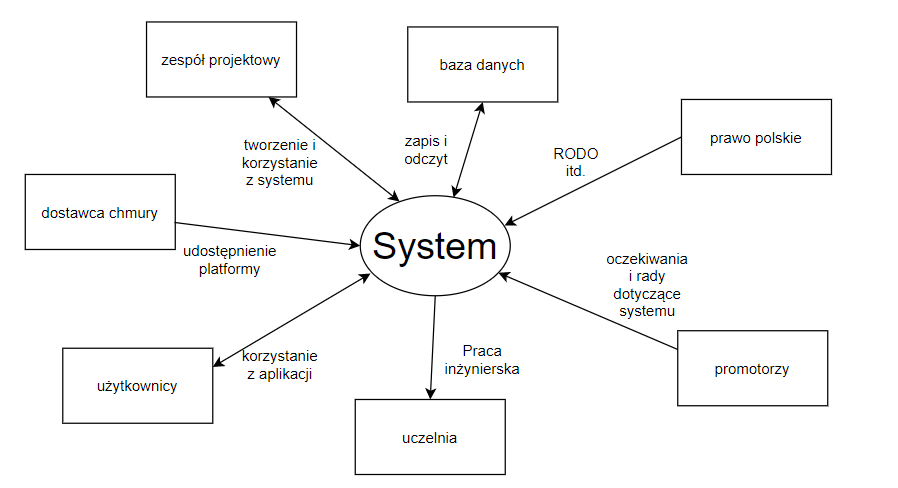
\includegraphics[width=15 cm, left]{system.png}
\section {Cele i odbiorcy systemu}
\subsection {Cele systemu}
Chcemy stworzyć nowe narzędzie do organizacji pracy z oryginalnym podejściem zaczerpniętym z systemów RPG,
 opartym na odkryciach w dziedzinie zarządzania energią\cite{Harward}.
 Chcemy, aby użytkownicy korzystający z naszego narzędzia nie zarządzali wyłącznie swoim czasem,
 ale także i energią, która jest równie ważna. Efektem będzie aplikacja internetowa.
 W przyszłości planujemy rozszerzyć system o aplikację mobilną oraz desktop'ową.
 Spodziewaną korzyścią będzie wzrost produktywności długoterminowej pośród użytkowników.
 Produktywność użytkowników moglibyśmy sprawdzać poprzez ankiety,
 porównujące czas poświęcony na zadania bez korzystania z systemu oraz z nim np. użytkownik skończył
 zaplanowane zadanie tydzień szybciej lub pracował przez 2 godziny dłużej niż bez korzystania z systemu.\\
\subsection {Udziałowcy (należy ponownie rozważyć)}
\begin{tabular}{|p{3cm}|p{11cm}|}
	\hline
	\multicolumn{2}{|l|}{\textbf{Karta Udziałowca}}\\
	\hline
	Identyfikator&UOB01\\
	\hline
	Nazwa&Zespół projektowy\\
	\hline
	Opis&Zespół projektowy tworzy oraz opiekuje się systemem\\
	\hline
	Typ udziałowca&Ożywiony, bezpośredni\\
	\hline
	Punkt widzenia&Perspektywa twórców systemu\\
	\hline
	Ograniczenia&Brak\\
	\hline
	Wymagania&\\
	\hline
	\end{tabular}\\
	\begin{tabular}{|p{3cm}|p{11cm}|}
	\hline
	\multicolumn{2}{|l|}{\textbf{Karta Udziałowca}}\\
	\hline
	Identyfikator&UOB02\\
	\hline
	Nazwa&Użytkownik końcowy\\
	\hline
	Opis&Przeciętny, finalny użytkownik korzystający z aplikacji\\
	\hline
	Typ udziałowca&Ożywiony, bezpośredni\\
	\hline
	Punkt widzenia&Perspektywa użytkownika\\
	\hline
	Ograniczenia&Nie ma dostępu do warstwy technicznej — bazy danych, kodu itp.\\
	\hline
	Wymagania&\\
	\hline
	\end{tabular}\\
	\begin{tabular}{|p{3cm}|p{11cm}|}
	\hline
	\multicolumn{2}{|l|}{\textbf{Karta Udziałowca}}\\
	\hline
	Identyfikator&UOB03\\
	\hline
	Nazwa&Sponsorzy\\
	\hline
	Opis&Osoba, która finansuje projekt i egzekwuje wymagania\\
	\hline
	Typ udziałowca&Ożywiony, bezpośredni\\
	\hline
	Punkt widzenia&Perspektywa ekonomiczna\\
	\hline
	Ograniczenia&Nie powinien narzucać technologii przy tworzeniu projektu\\
	\hline
	Wymagania&\\
	\hline
	\end{tabular}\\
	\begin{tabular}{|p{3cm}|p{11cm}|}
	\hline
	\multicolumn{2}{|l|}{\textbf{Karta Udziałowca}}\\
	\hline
	Identyfikator&UOB04\\
	\hline
	Nazwa&Wydawca\\
	\hline
	Opis&Osoba, która jest odpowiedzialna za sfinalizowanie projektu i wypuszczenie go na rynek\\
	\hline
	Typ udziałowca&Ożywiony, bezpośredni\\
	\hline
	Punkt widzenia&Perspektywa ekonomiczna\\
	\hline
	Ograniczenia&Nie powinien narzucać technologii przy tworzeniu projektu\\
	\hline
	Wymagania&\\
	\hline
	\end{tabular}\\
	\begin{tabular}{|p{3cm}|p{11cm}|}
	\hline
	\multicolumn{2}{|l|}{\textbf{Karta Udziałowca}}\\
	\hline
	Identyfikator&UOB05\\
	\hline
	Nazwa&Promotorzy\\
	\hline
	Opis&Doradcy w sprawach dotyczących projektu\\
	\hline
	Typ udziałowca&Ożywiony, bezpośredni\\
	\hline
	Punkt widzenia&Perspektywa twórców projektu\\
	\hline
	Ograniczenia&Nie zawsze dostępni\\
	\hline
	Wymagania&\\
	\hline
	\end{tabular}\\
	\begin{tabular}{|p{3cm}|p{11cm}|}
	\hline
	\multicolumn{2}{|l|}{\textbf{Karta Udziałowca}}\\
	\hline
	Identyfikator&UNB01\\
	\hline
	Nazwa&Media\\
	\hline
	Opis&Strony internetowe, reklamy, artykuły, audycje itp.\\
	\hline
	Typ udziałowca&Nieożywiony, bezpośredni\\
	\hline
	Punkt widzenia&Perspektywa ekonomiczna\\
	\hline
	Ograniczenia&Zero wpływu na budowę projektu\\
	\hline
	Wymagania&\\
	\hline
	\end{tabular}\\
	\begin{tabular}{|p{3cm}|p{11cm}|}
	\hline
	\multicolumn{2}{|l|}{\textbf{Karta Udziałowca}}\\
	\hline
	Identyfikator&UNB02\\
	\hline
	Nazwa&Baza danych\\
	\hline
	Opis&Jedna, wspólna baza danych na cały system\\
	\hline
	Typ udziałowca&Nieożywiony, bezpośredni\\
	\hline
	Punkt widzenia&Perspektywa techniczna\\
	\hline
	Ograniczenia&Skończona ilość pamięci do przechowywania informacji\\
	\hline
	Wymagania&\\
	\hline
	\end{tabular}\\
	\begin{tabular}{|p{3cm}|p{11cm}|}
	\hline
	\multicolumn{2}{|l|}{\textbf{Karta Udziałowca}}\\
	\hline
	Identyfikator&UNB03\\
	\hline
	Nazwa&Prawo polskie\\
	\hline
	Opis&Zgodnie z RODO mamy obowiązek dbać o bezpieczeństwo danych osobowych wszystkich użytkowników\\
	\hline
	Typ udziałowca&Nieożywiony, bezpośredni\\
	\hline
	Punkt widzenia&Perspektywa prawna\\
	\hline
	Ograniczenia&Brak\\
	\hline
	Wymagania&\\
	\hline
	\end{tabular}\\
	\begin{tabular}{|p{3cm}|p{11cm}|}
	\hline
	\multicolumn{2}{|l|}{\textbf{Karta Udziałowca}}\\
	\hline
	Identyfikator&UNB04\\
	\hline
	Nazwa&Dostawca usług chmurowych\\
	\hline
	Opis&Serwer w chmurze odpowiedzialny za przetwarzanie wszystkich żądań pomiędzy serwisami i użytkownikami końcowymi\\
	\hline
	Typ udziałowca&Nieożywiony, bezpośredni\\
	\hline
	Punkt widzenia&Perspektywa techniczna\\
	\hline
	Ograniczenia& Sprzętowe, specyfikacja sprzętu (np. moc procesora serwerowego, przepustowość Internetu)\\
	\hline
	Wymagania&\\
	\hline
	\end{tabular}\\
\subsection {Grupa docelowa}
Grupa docelowa to osoby, które chcą poprawić swoją higienę pracy, chcą stać się systematyczni, uniknąć przepracowania. (ładniej opisać)
\chapter {Analiza}

\section {Wymagania (w trakcie ponownego rozważania)}
\subsection {Wymagania ogólne i dziedzinowe}
		\begin{tabular}{|p{3cm}|p{2cm}|p{2cm}|p{6cm}|}
		\hline
		\multicolumn{4}{|p{12 cm}|}{Karta Wymagania}\\
		\hline
		Identyfikator: & W01 & Priorytet: & M — must (musi być)\\
		\hline
		Nazwa & \multicolumn{3}{|p{10 cm}|}{Zwiększenie efektywności pracy użytkowników systemu}\\
		\hline
		Opis & \multicolumn{3}{|p{10 cm}|}{Końcowy produkt systemu ma za zadanie zwiększać produktywność jego użytkowników, weryfikowane jest to na podstawie prac z Harvardu i user feedbacku w postaci ankiet.}\\
		\hline
		Udziałowiec & \multicolumn{3}{|p{10 cm}|}{Wydawca, Użytkownik końcowy}\\
		\hline
		Wymagania powiązane & \multicolumn{3}{|p{10 cm}|}{Brak}\\
		\hline
		\end{tabular}\\
		\begin{tabular}{|p{3cm}|p{2cm}|p{2cm}|p{6cm}|}
		\hline
		\multicolumn{4}{|p{12 cm}|}{Karta Wymagania}\\
		\hline
		Identyfikator: & W01 & Priorytet: &  M — must (musi być)\\
		\hline
		Nazwa & \multicolumn{3}{|p{10 cm}|}{System skórek}\\
		\hline
		Opis & \multicolumn{3}{|p{10 cm}|}{Produkt będzie zarabiał na sprzedaży skórek (alternatywna oprawa graficzna i personalizacja systemu pracy)}\\
		\hline
		Udziałowiec & \multicolumn{3}{|p{10 cm}|}{Wydawca, Sponsorzy}\\
		\hline
		Wymagania powiązane & \multicolumn{3}{|p{10 cm}|}{Brak}\\
		\hline
		\end{tabular}\\
	\subsection {Wymagania funkcjonalne}
	\begin{itemize}
		\item Nazwa funkcji/usługi\\
		\begin{tabular}{|p{3cm}|p{2cm}|p{2cm}|p{6cm}|}
		\hline
		\multicolumn{4}{|p{12 cm}|}{Karta Wymagania}\\
		\hline
		Identyfikator: & F01 & Priorytet: & M — must (musi być)\\
		\hline
		Nazwa & \multicolumn{3}{|p{10 cm}|}{System Autoryzacji użytkownika}\\
		\hline
		Opis & \multicolumn{3}{|p{10 cm}|}{Jako użytkownik muszę mieć możliwość zarejestrowania się w serwisie i późniejszego logowania się}\\
		\hline
		Kryteria akceptacji & \multicolumn{3}{|p{10 cm}|}{Bezpieczny system autoryzacji zabezpieczony przed atakami na bazę danych, potwierdzenie maila po rejestracji,  jedno konta na 1 mail}\\
		\hline
		Dane wejściowe & \multicolumn{3}{|p{10 cm}|}{Brak}\\
		\hline
		Warunki początkowe & \multicolumn{3}{|p{10 cm}|}{Brak}\\
		\hline
		Warunki końcowe & \multicolumn{3}{|p{10 cm}|}{Brak}\\
		\hline
		Sytuacje wyjątkowe & \multicolumn{3}{|p{10 cm}|}{Brak}\\
		\hline
		Szczegóły implementacji & \multicolumn{3}{|p{10 cm}|}{Brak}\\
		\hline
		Udziałowiec & \multicolumn{3}{|p{10 cm}|}{Użytkownik końcowy, Zespół projektowy}\\
		\hline
		Wymagania powiązane & \multicolumn{3}{|p{10 cm}|}{Brak}\\
		\hline
		\end{tabular}\\
		\begin{tabular}{|p{3cm}|p{2cm}|p{2cm}|p{6cm}|}
		\hline
		\multicolumn{4}{|p{12 cm}|}{Karta Wymagania}\\
		\hline
		Identyfikator: & F02 & Priorytet: & M — must (musi być)\\
		\hline
		Nazwa & \multicolumn{3}{|p{10 cm}|}{System rang użytkowników}\\
		\hline
		Opis & \multicolumn{3}{|p{10 cm}|}{Jako użytkownik podczas postępowania w używaniu aplikacji chciałbym być przypisywany do różnych rang}\\
		\hline
		Kryteria akceptacji & \multicolumn{3}{|p{10 cm}|}{Przypisywanie rangi do danego użytkownika oraz obliczanie jego statystyk na podstawie wykonywanych projektów}\\
		\hline
		Dane wejściowe & \multicolumn{3}{|p{10 cm}|}{Brak}\\
		\hline
		Warunki początkowe & \multicolumn{3}{|p{10 cm}|}{Brak}\\
		\hline
		Warunki końcowe & \multicolumn{3}{|p{10 cm}|}{Brak}\\
		\hline
		Sytuacje wyjątkowe & \multicolumn{3}{|p{10 cm}|}{Brak}\\
		\hline
		Szczegóły implementacji & \multicolumn{3}{|p{10 cm}|}{Brak}\\
		\hline
		Udziałowiec & \multicolumn{3}{|p{10 cm}|}{Użytkownik końcowy, Zespół projektowy}\\
		\hline
		Wymagania powiązane & \multicolumn{3}{|p{10 cm}|}{Brak}\\
		\hline
		\end{tabular}\\
		\begin{tabular}{|p{3cm}|p{2cm}|p{2cm}|p{6cm}|}
		\hline
		\multicolumn{4}{|p{12 cm}|}{Karta Wymagania}\\
		\hline
		Identyfikator: & F03 & Priorytet: & M — must (musi być)\\
		\hline
		Nazwa & \multicolumn{3}{|p{10 cm}|}{System zarządzania energią  użytkownika}\\
		\hline
		Opis & \multicolumn{3}{|p{10 cm}|}{Jako użytkownik chcę, żeby aplikacja śledziła moje zasoby energetyczne i podpowiadała, jak mogę nimi lepiej zarządzać}\\
		\hline
		Kryteria akceptacji & \multicolumn{3}{|p{10 cm}|}{Zmiana zasobów energii użytkownika przy wykonywaniu konkretnych projektów lub przerw}\\
		\hline
		Dane wejściowe & \multicolumn{3}{|p{10 cm}|}{Brak}\\
		\hline
		Warunki początkowe & \multicolumn{3}{|p{10 cm}|}{Brak}\\
		\hline
		Warunki końcowe & \multicolumn{3}{|p{10 cm}|}{Brak}\\
		\hline
		Sytuacje wyjątkowe & \multicolumn{3}{|p{10 cm}|}{Brak}\\
		\hline
		Szczegóły implementacji & \multicolumn{3}{|p{10 cm}|}{Brak}\\
		\hline
		Udziałowiec & \multicolumn{3}{|p{10 cm}|}{Użytkownik końcowy, Zespół projektowy}\\
		\hline
		Wymagania powiązane & \multicolumn{3}{|p{10 cm}|}{Brak}\\
		\hline
		\end{tabular}\\
		\begin{tabular}{|p{3cm}|p{2cm}|p{2cm}|p{6cm}|}
		\hline
		\multicolumn{4}{|p{12 cm}|}{Karta Wymagania}\\
		\hline
		Identyfikator: & F04 & Priorytet: & M — must (musi być)\\
		\hline
		Nazwa & \multicolumn{3}{|p{10 cm}|}{System zarządzania projektami użytkowników}\\
		\hline
		Opis & \multicolumn{3}{|p{10 cm}|}{Jako użytkownik chciałbym mieć możliwość dodawania, usuwania i śledzenia projektów lub zadań}\\
		\hline
		Kryteria akceptacji & \multicolumn{3}{|p{10 cm}|}{Użytkownik ma możliwość dodawania, usuwania i śledzenia projektów przez siebie stworzonych}\\
		\hline
		Dane wejściowe & \multicolumn{3}{|p{10 cm}|}{Brak}\\
		\hline
		Warunki początkowe & \multicolumn{3}{|p{10 cm}|}{Brak}\\
		\hline
		Warunki końcowe & \multicolumn{3}{|p{10 cm}|}{Brak}\\
		\hline
		Sytuacje wyjątkowe & \multicolumn{3}{|p{10 cm}|}{Brak}\\
		\hline
		Szczegóły implementacji & \multicolumn{3}{|p{10 cm}|}{Brak}\\
		\hline
		Udziałowiec & \multicolumn{3}{|p{10 cm}|}{Użytkownik końcowy, Zespół projektowy}\\
		\hline
		Wymagania powiązane & \multicolumn{3}{|p{10 cm}|}{Brak}\\
		\hline
		\end{tabular}\\
		\begin{tabular}{|p{3cm}|p{2cm}|p{2cm}|p{6cm}|}
		\hline
		\multicolumn{4}{|p{12 cm}|}{Karta Wymagania}\\
		\hline
		Identyfikator: & F05 & Priorytet: & M — must (musi być)\\
		\hline
		Nazwa & \multicolumn{3}{|p{10 cm}|}{Bullet Journal}\\
		\hline
		Opis & \multicolumn{3}{|p{10 cm}|}{Jako użytkownik chcę mieć możliwość rozplanowania zadań na dni oraz zobaczenia ich rozłożonych w czasie na tablicy lub w postaci kalendarza}\\
		\hline
		Kryteria akceptacji & \multicolumn{3}{|p{10 cm}|}{Użytkownik może dodawać swoje zadania wraz z datami ich wykonania, które zostają wizualizowane w postaci tablicy lub kalendarza}\\
		\hline
		Dane wejściowe & \multicolumn{3}{|p{10 cm}|}{Brak}\\
		\hline
		Warunki początkowe & \multicolumn{3}{|p{10 cm}|}{Brak}\\
		\hline
		Warunki końcowe & \multicolumn{3}{|p{10 cm}|}{Brak}\\
		\hline
		Sytuacje wyjątkowe & \multicolumn{3}{|p{10 cm}|}{Brak}\\
		\hline
		Szczegóły implementacji & \multicolumn{3}{|p{10 cm}|}{Brak}\\
		\hline
		Udziałowiec & \multicolumn{3}{|p{10 cm}|}{Użytkownik końcowy, Zespół projektowy}\\
		\hline
		Wymagania powiązane & \multicolumn{3}{|p{10 cm}|}{Brak}\\
		\hline
		\end{tabular}\\
		\begin{tabular}{|p{3cm}|p{2cm}|p{2cm}|p{6cm}|}
		\hline
		\multicolumn{4}{|p{12 cm}|}{Karta Wymagania}\\
		\hline
		Identyfikator: & F06 & Priorytet: & C – could \\
		\hline
		Nazwa & \multicolumn{3}{|p{10 cm}|}{System osiągnięć użytkownika}\\
		\hline
		Opis & \multicolumn{3}{|p{10 cm}|}{Jako użytkownik chciałbym co jakiś czas być nagradzany za osiągnięcia przy dochodzeniu do kamieni milowych podczas korzystania z aplikacji}\\
		\hline
		Kryteria akceptacji & \multicolumn{3}{|p{10 cm}|}{Użytkownik otrzymuje osiągnięcia za przekroczenie pewnych kamieni milowych}\\
		\hline
		Dane wejściowe & \multicolumn{3}{|p{10 cm}|}{Brak}\\
		\hline
		Warunki początkowe & \multicolumn{3}{|p{10 cm}|}{Brak}\\
		\hline
		Warunki końcowe & \multicolumn{3}{|p{10 cm}|}{Brak}\\
		\hline
		Sytuacje wyjątkowe & \multicolumn{3}{|p{10 cm}|}{Brak}\\
		\hline
		Szczegóły implementacji & \multicolumn{3}{|p{10 cm}|}{Brak}\\
		\hline
		Udziałowiec & \multicolumn{3}{|p{10 cm}|}{Użytkownik końcowy, Zespół projektowy}\\
		\hline
		Wymagania powiązane & \multicolumn{3}{|p{10 cm}|}{Brak}\\
		\hline
		\end{tabular}\\
		\begin{tabular}{|p{3cm}|p{2cm}|p{2cm}|p{6cm}|}
		\hline
		\multicolumn{4}{|p{12 cm}|}{Karta Wymagania}\\
		\hline
		Identyfikator: & F07 & Priorytet: & C – could\\
		\hline
		Nazwa & \multicolumn{3}{|p{10 cm}|}{System rankingowy użytkowników}\\
		\hline
		Opis & \multicolumn{3}{|p{10 cm}|}{Jako użytkownik chciałbym mieć dostęp do tablic rankingowych, gdzie mógłbym porównywać swoje osiągnięcia z innymi użytkownikami.}\\
		\hline
		Kryteria akceptacji & \multicolumn{3}{|p{10 cm}|}{Użytkownik jest w stanie sprawdzić swoją pozycję w rankingu dotyczącą danego projektu}\\
		\hline
		Dane wejściowe & \multicolumn{3}{|p{10 cm}|}{Brak}\\
		\hline
		Warunki początkowe & \multicolumn{3}{|p{10 cm}|}{Brak}\\
		\hline
		Warunki końcowe & \multicolumn{3}{|p{10 cm}|}{Brak}\\
		\hline
		Sytuacje wyjątkowe & \multicolumn{3}{|p{10 cm}|}{Brak}\\
		\hline
		Szczegóły implementacji & \multicolumn{3}{|p{10 cm}|}{Brak}\\
		\hline
		Udziałowiec & \multicolumn{3}{|p{10 cm}|}{Użytkownik końcowy, Zespół projektowy}\\
		\hline
		Wymagania powiązane & \multicolumn{3}{|p{10 cm}|}{Brak}\\
		\hline
		\end{tabular}\\
		\begin{tabular}{|p{3cm}|p{2cm}|p{2cm}|p{6cm}|}
		\hline
		\multicolumn{4}{|p{12 cm}|}{Karta Wymagania}\\
		\hline
		Identyfikator: & F08 & Priorytet: & C – could \\
		\hline
		Nazwa & \multicolumn{3}{|p{10 cm}|}{System znajomych użytkowników}\\
		\hline
		Opis & \multicolumn{3}{|p{10 cm}|}{Jako użytkownik chciałbym móc dodawać innych użytkowników do swojej listy znajomych, żeby sprawdzać ich postępy}\\
		\hline
		Kryteria akceptacji & \multicolumn{3}{|p{10 cm}|}{Użytkownik może dodawaj znajomych, wyświetlanych w formie listy, u których może sprawdzać ich postępy}\\
		\hline
		Dane wejściowe & \multicolumn{3}{|p{10 cm}|}{Brak}\\
		\hline
		Warunki początkowe & \multicolumn{3}{|p{10 cm}|}{Brak}\\
		\hline
		Warunki końcowe & \multicolumn{3}{|p{10 cm}|}{Brak}\\
		\hline
		Sytuacje wyjątkowe & \multicolumn{3}{|p{10 cm}|}{Brak}\\
		\hline
		Szczegóły implementacji & \multicolumn{3}{|p{10 cm}|}{Brak}\\
		\hline
		Udziałowiec & \multicolumn{3}{|p{10 cm}|}{Użytkownik końcowy, Zespół projektowy}\\
		\hline
		Wymagania powiązane & \multicolumn{3}{|p{10 cm}|}{Brak}\\
		\hline
		\end{tabular}\\
		\begin{tabular}{|p{3cm}|p{2cm}|p{2cm}|p{6cm}|}
		\hline
		\multicolumn{4}{|p{12 cm}|}{Karta Wymagania}\\
		\hline
		Identyfikator: & F09 & Priorytet: & C – could\\
		\hline
		Nazwa & \multicolumn{3}{|p{10 cm}|}{Energy Assistant}\\
		\hline
		Opis & \multicolumn{3}{|p{10 cm}|}{Jako użytkownik chciałbym, żeby moje rzeczywiste poziomy energii były lepiej rozpoznawane.}\\
		\hline
		Kryteria akceptacji & \multicolumn{3}{|p{10 cm}|}{Użytkownik zależnie jaki prowadzi tryb życia bądź w zależności od jego warunków fizycznych, jak i psychicznych miałby dostosowywaną ilość energii na dany dzień}\\
		\hline
		Dane wejściowe & \multicolumn{3}{|p{10 cm}|}{Brak}\\
		\hline
		Warunki początkowe & \multicolumn{3}{|p{10 cm}|}{Brak}\\
		\hline
		Warunki końcowe & \multicolumn{3}{|p{10 cm}|}{Brak}\\
		\hline
		Sytuacje wyjątkowe & \multicolumn{3}{|p{10 cm}|}{Brak}\\
		\hline
		Szczegóły implementacji & \multicolumn{3}{|p{10 cm}|}{Brak}\\
		\hline
		Udziałowiec & \multicolumn{3}{|p{10 cm}|}{Użytkownik końcowy, Zespół projektowy}\\
		\hline
		Wymagania powiązane & \multicolumn{3}{|p{10 cm}|}{Brak}\\
		\hline
		\end{tabular}\\
		\begin{tabular}{|p{3cm}|p{2cm}|p{2cm}|p{6cm}|}
		\hline
		\multicolumn{4}{|p{12 cm}|}{Karta Wymagania}\\
		\hline
		Identyfikator: & F10 & Priorytet: & C – could\\
		\hline
		Nazwa & \multicolumn{3}{|p{10 cm}|}{Elastic Habits}\\
		\hline
		Opis & \multicolumn{3}{|p{10 cm}|}{Jako użytkownik chciałbym móc podzielić swoje zadanie na różne poziomy trudności.}\\
		\hline
		Kryteria akceptacji & \multicolumn{3}{|p{10 cm}|}{Użytkownik może wybrać z dany poziom trudności zadania, by wyrobić sobie nawyk wykonywania go.}\\
		\hline
		Dane wejściowe & \multicolumn{3}{|p{10 cm}|}{Brak}\\
		\hline
		Warunki początkowe & \multicolumn{3}{|p{10 cm}|}{Brak}\\
		\hline
		Warunki końcowe & \multicolumn{3}{|p{10 cm}|}{Brak}\\
		\hline
		Sytuacje wyjątkowe & \multicolumn{3}{|p{10 cm}|}{Brak}\\
		\hline
		Szczegóły implementacji & \multicolumn{3}{|p{10 cm}|}{Brak}\\
		\hline
		Udziałowiec & \multicolumn{3}{|p{10 cm}|}{Użytkownik końcowy, Zespół projektowy}\\
		\hline
		Wymagania powiązane & \multicolumn{3}{|p{10 cm}|}{Brak}\\
		\hline
		\end{tabular}\\
		\item Interfejs z otoczeniem\\
		\begin{tabular}{|p{3cm}|p{2cm}|p{2cm}|p{6cm}|}
		\hline
		\multicolumn{4}{|p{12 cm}|}{Karta Wymagania}\\
		\hline
		Identyfikator: & I01 & Priorytet: & M – must (musi być)\\
		\hline
		Nazwa & \multicolumn{3}{|p{10 cm}|}{Integracja mikro serwisów}\\
		\hline
		Opis & \multicolumn{3}{|p{10 cm}|}{Nasz projekt strukturalnie będzie zbudowany z wielu mikro serwisów i wymagana jest integracja między nimi (komunikatywność).}\\
		\hline
		Kryteria akceptacji & \multicolumn{3}{|p{10 cm}|}{Funkcje w każdym serwisie umożliwiające komunikowanie się z innymi serwisami}\\
		\hline
		Dane wejściowe & \multicolumn{3}{|p{10 cm}|}{Brak}\\
		\hline
		Warunki początkowe & \multicolumn{3}{|p{10 cm}|}{Brak}\\
		\hline
		Warunki końcowe & \multicolumn{3}{|p{10 cm}|}{Brak}\\
		\hline
		Sytuacje wyjątkowe & \multicolumn{3}{|p{10 cm}|}{Brak}\\
		\hline
		Szczegóły implementacji & \multicolumn{3}{|p{10 cm}|}{Brak}\\
		\hline
		Udziałowiec & \multicolumn{3}{|p{10 cm}|}{Zespół projektowy}\\
		\hline
		Wymagania powiązane & \multicolumn{3}{|p{10 cm}|}{Brak}\\
		\hline
		\end{tabular}\\
		\begin{tabular}{|p{3cm}|p{2cm}|p{2cm}|p{6cm}|}
		\hline
		\multicolumn{4}{|p{12 cm}|}{Karta Wymagania}\\
		\hline
		Identyfikator: & I02 & Priorytet: & M – must (musi być)\\
		\hline
		Nazwa & \multicolumn{3}{|p{10 cm}|}{Baza danych}\\
		\hline
		Opis & \multicolumn{3}{|p{10 cm}|}{Jedna zintegrowana baza danych dla wszystkich serwisów}\\
		\hline
		Kryteria akceptacji & \multicolumn{3}{|p{10 cm}|}{Baza danych w MongoDB która będzie obsługiwać wszystkie mikro serwisy projektu, będzie posiadała dane użytkowników i wszystkiego, co jest związane z aplikacją.}\\
		\hline
		Dane wejściowe & \multicolumn{3}{|p{10 cm}|}{Brak}\\
		\hline
		Warunki początkowe & \multicolumn{3}{|p{10 cm}|}{Brak}\\
		\hline
		Warunki końcowe & \multicolumn{3}{|p{10 cm}|}{Brak}\\
		\hline
		Sytuacje wyjątkowe & \multicolumn{3}{|p{10 cm}|}{Brak}\\
		\hline
		Szczegóły implementacji & \multicolumn{3}{|p{10 cm}|}{Brak}\\
		\hline
		Udziałowiec & \multicolumn{3}{|p{10 cm}|}{Zespół projektowy}\\
		\hline
		Wymagania powiązane & \multicolumn{3}{|p{10 cm}|}{Brak}\\
		\hline
		\end{tabular}\\
	\end{itemize}
	\subsection {Wymagania poza funkcjonalne}
	\begin{tabular}{|p{3cm}|p{2cm}|p{2cm}|p{6cm}|}
		\hline
		\multicolumn{4}{|p{12 cm}|}{Karta Wymagania}\\
		\hline
		Identyfikator: & NF01 & Priorytet: & M – must (musi być)\\
		\hline
		Nazwa & \multicolumn{3}{|p{10 cm}|}{C\#}\\
		\hline
		Opis & \multicolumn{3}{|p{10 cm}|}{Serwisy backend'owe powinny być napisane w C\#}\\
		\hline
		Udziałowiec & \multicolumn{3}{|p{10 cm}|}{Zespół projektowy, Wydawca}\\
		\hline
		Wymagania powiązane & \multicolumn{3}{|p{10 cm}|}{Brak}\\
		\hline
		\end{tabular}\\
		\begin{tabular}{|p{3cm}|p{2cm}|p{2cm}|p{6cm}|}
		\hline
		\multicolumn{4}{|p{12 cm}|}{Karta Wymagania}\\
		\hline
		Identyfikator: & NF02 & Priorytet: & M – must (musi być)\\
		\hline
		Nazwa & \multicolumn{3}{|p{10 cm}|}{React}\\
		\hline
		Opis & \multicolumn{3}{|p{10 cm}|}{Serwis frontend'owy powinien być napisany, korzystając z biblioteki React.}\\
		\hline
		Udziałowiec & \multicolumn{3}{|p{10 cm}|}{Zespół projektowy, Wydawca}\\
		\hline
		Wymagania powiązane & \multicolumn{3}{|p{10 cm}|}{Brak}\\
		\hline
		\end{tabular}\\
		\begin{tabular}{|p{3cm}|p{2cm}|p{2cm}|p{6cm}|}
		\hline
		\multicolumn{4}{|p{12 cm}|}{Karta Wymagania}\\
		\hline
		Identyfikator: & NF03 & Priorytet: & M – must (musi być)\\
		\hline
		Nazwa & \multicolumn{3}{|p{10 cm}|}{Czas wdrożenia}\\
		\hline
		Opis & \multicolumn{3}{|p{10 cm}|}{System należy wdrożyć do końca semestru zimowego 2020/2021}\\
		\hline
		Udziałowiec & \multicolumn{3}{|p{10 cm}|}{Zespół projektowy, Promotorzy, Uczelnia, Wydawca}\\
		\hline
		Wymagania powiązane & \multicolumn{3}{|p{10 cm}|}{Brak}\\
		\hline
		\end{tabular}\\
		\begin{tabular}{|p{3cm}|p{2cm}|p{2cm}|p{6cm}|}
		\hline
		\multicolumn{4}{|p{12 cm}|}{Karta Wymagania}\\
		\hline
		Identyfikator: & NF04 & Priorytet: & M – must (musi być)\\
		\hline
		Nazwa & \multicolumn{3}{|p{10 cm}|}{System powinien być dostępny 24 godziny na dobę, 7 dni w tygodniu}\\
		\hline
		Opis & \multicolumn{3}{|p{10 cm}|}{Dostęp do systemu powinien być umożliwiony w dowolnej chwili danego dnia}\\
		\hline
		Udziałowiec & \multicolumn{3}{|p{10 cm}|}{Zespół projektowy, Użytkownik końcowy, Wydawca}\\
		\hline
		Wymagania powiązane & \multicolumn{3}{|p{10 cm}|}{Brak}\\
		\hline
		\end{tabular}\\
	\subsection {Wymagania na środowisko docelowe}
	\begin{tabular}{|p{3cm}|p{2cm}|p{2cm}|p{6cm}|}
		\hline
		\multicolumn{4}{|p{12 cm}|}{Karta Wymagania}\\
		\hline
		Identyfikator: & ŚD01 & Priorytet: & M – must (musi być)\\
		\hline
		Nazwa & \multicolumn{3}{|p{10 cm}|}{Kompatybilność przeglądarek}\\
		\hline
		Opis & \multicolumn{3}{|p{10 cm}|}{Produkt końcowy musi być kompatybilny z 3 najnowszymi wersjami popularnych przeglądarek}\\
		\hline
		Kryteria akceptacji & \multicolumn{3}{|p{10 cm}|}{System kompatybilny z 3 najnowszymi wersjami przeglądarek Google Chrome i Mozilla Firefox}\\
		\hline
		Udziałowiec & \multicolumn{3}{|p{10 cm}|}{Zespół projektowy, Użytkownik końcowy, Wydawca}\\
		\hline
		Wymagania powiązane & \multicolumn{3}{|p{10 cm}|}{Brak}\\
		\hline
		\end{tabular}\\
	\section {Wymagania jakościowe i inne}
	\begin{itemize}
		\item System szyfrowania danych użytkowników: szyfrowanie transmisji, haseł i ciasteczek
		\item Wsparcie dla ostatnich trzech wersji Google Chrome i Mozilla Firefox
		\item System dostępny 24 godziny na dobę z wyłączeniem prac technicznych
		\item System ma być łatwy w obsłudze – średnio 5 kliknięć na wykonanie dowolnej 
	\end{itemize}
\section{Przypadki użycia oraz diagramy (w trakcie przerabiania i tworzenia nowych)}
\subsection{Przypadki użycia}
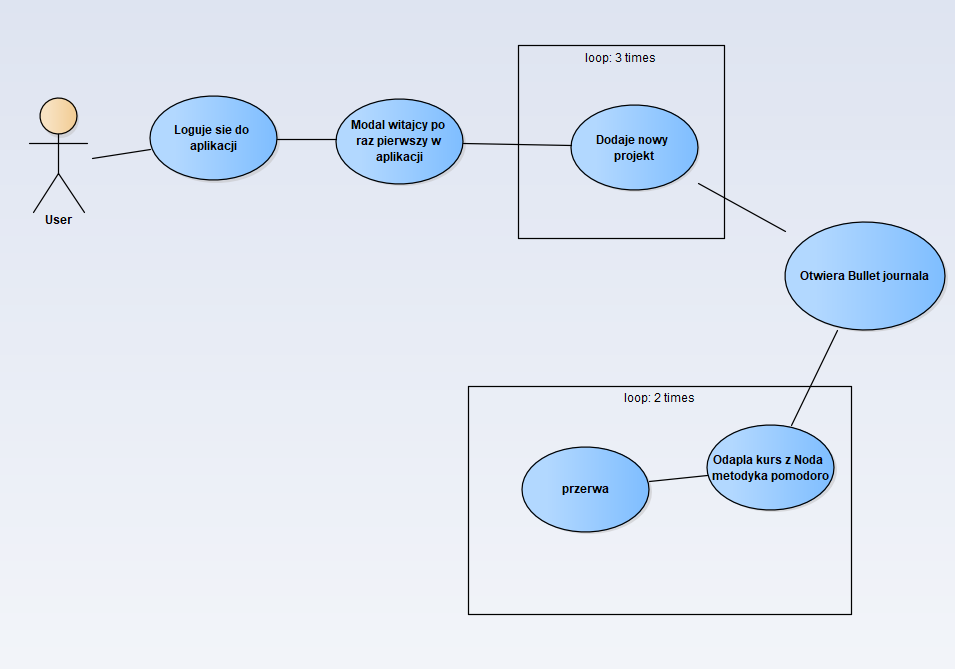
\includegraphics[width=\textwidth, height=9cm]{usecase1.png}\\
\vspace{0.5cm}
Use case 1\\
\vspace{0.5cm}
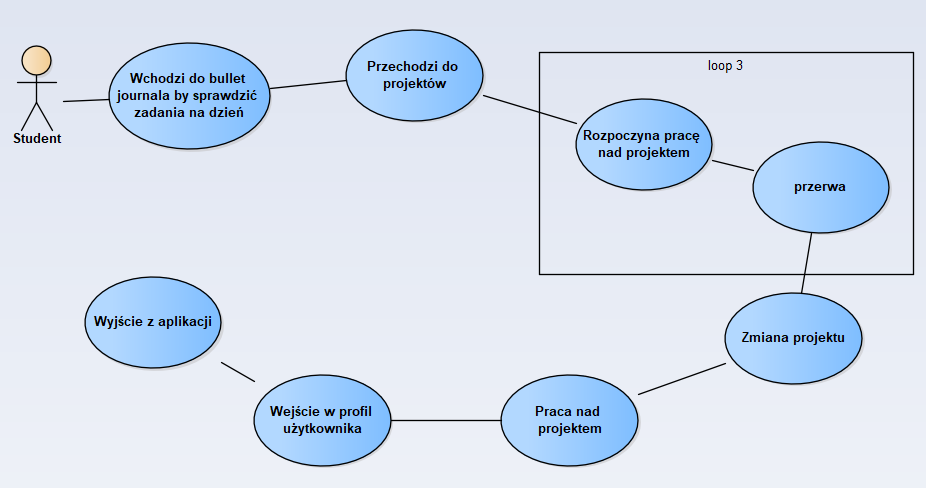
\includegraphics[width=\textwidth, height=9cm]{usecase2.png}\\
\vspace{0.5cm}
Use case 2\\
\vspace{0.5cm}
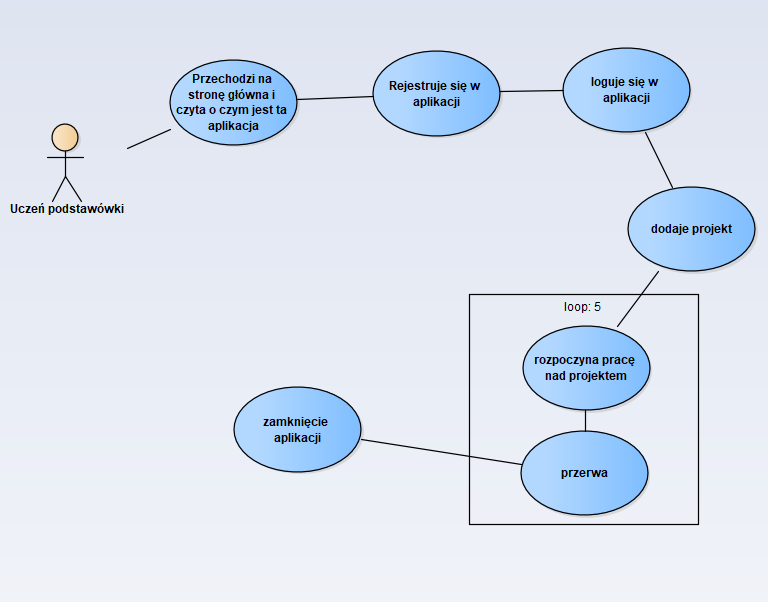
\includegraphics[width=\textwidth, height=9cm]{usecase3.png}\\
Use case 3\\
\vspace{0.5cm}
\subsection{Diagramy}
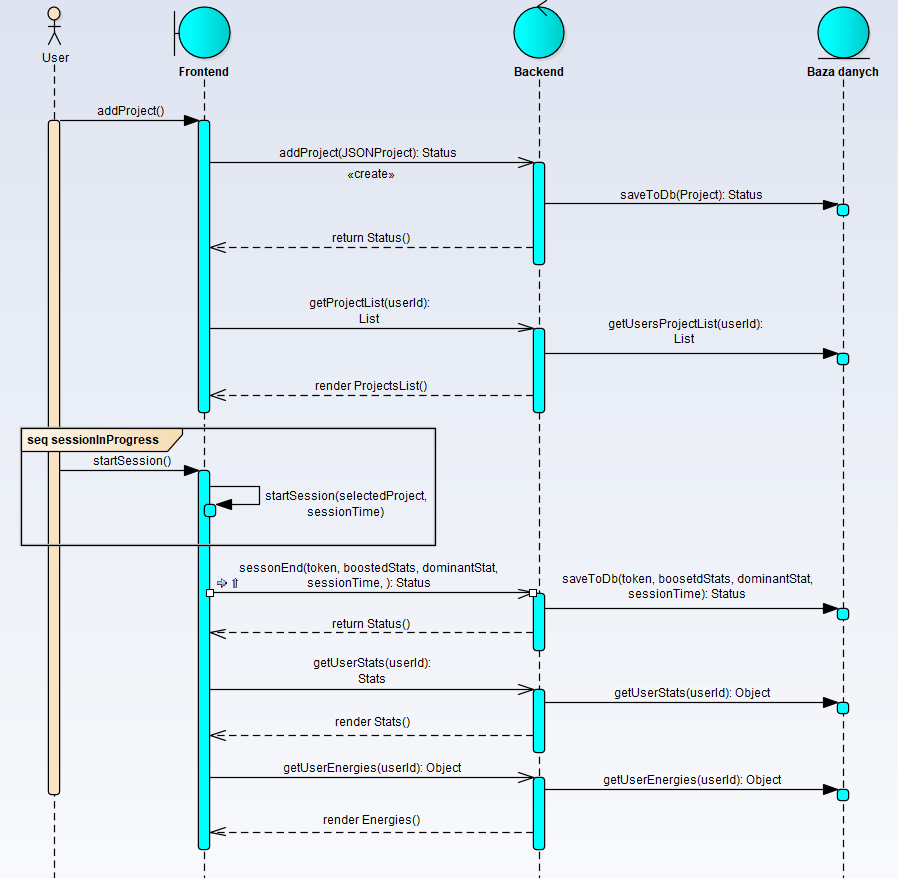
\includegraphics[width=\textwidth, height=9cm]{sekwencji.png}\\
Diagram sekwencji\\
\vspace{0.5cm}
\chapter {Planowanie}
\section{Metodyka pracy}
Po dłuższym namyśle zdecydowaliśmy, że dobrym dla nas podejściem byłoby podążanie sprintami z metodologii Scrum
 oraz posiadanie tablicy zadań z metodologii Kanban\cite{agile}.
 Sprinty wymuszają na nas ciągłą, stałą pracę, by co tydzień wypuszczać nowe wersje naszego systemu.
 Zapewnia to stałą motywację do pracy, by nie osiągnąć punktu długotrwałej stagnacji w projekcie.
 Tablica zadań z metodologii Kanban pozwala nam na jasne podzielenie zadań w zespole projektowym
 oraz ułatwia określenie, w jakim stopniu dane zadanie jest wykonane.
 Wybraliśmy tę metodykę ze względu na fakt, że nasz system jest dość nowatorski w swojej kategorii,
 przez co wymaga stałej weryfikacji przez użytkowników.
\section{Narzędzia}
Opisanie narzędzi wykorzystanych do tworzenia projektu (Slack, Azure DevOps, Gcloud itd.)
\section{Technologie}
		\begin{itemize}
			\item React/Redux/MUI — frontend
			\item .NET — Backend
			\item MongoDB/Postgres — baza danych
		\end{itemize}

\chapter {Projektowanie}

\section {Architektura projektu}
\subsection{Frontend} 
\subsection{Backend}
\subsection{Baza Danych}
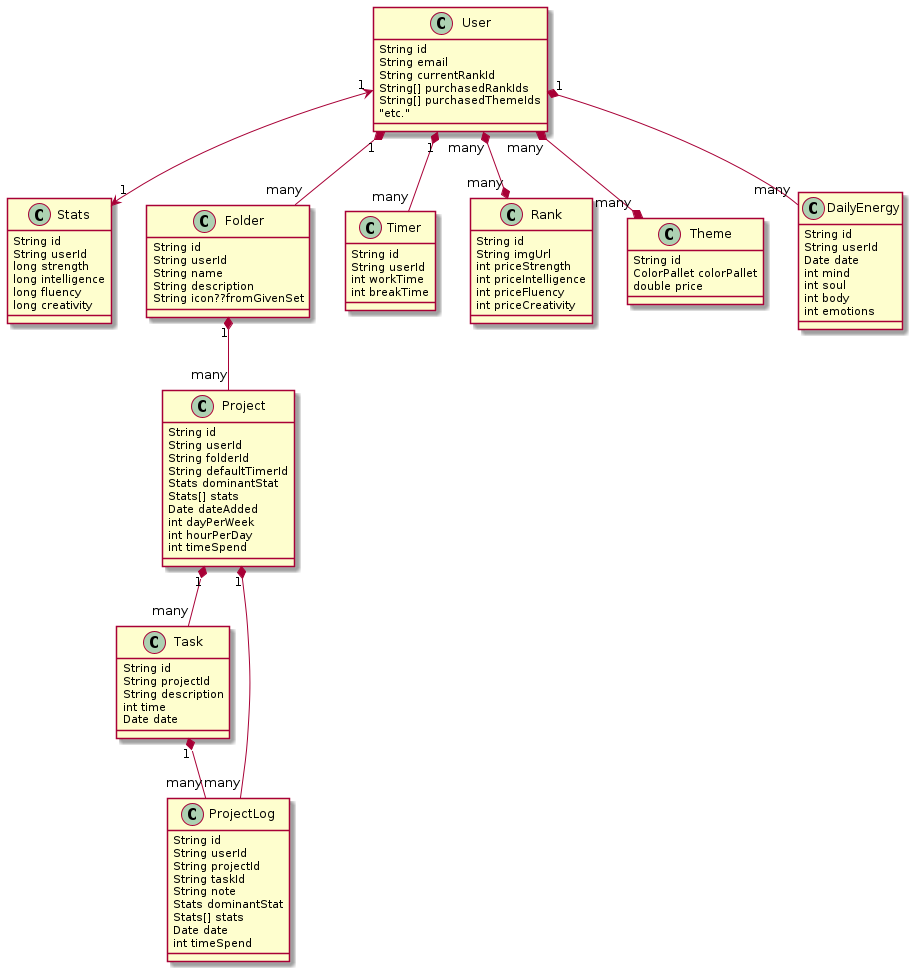
\includegraphics[width=\textwidth, height=10cm]{gamitude database model.png}\\
Schemat bazy danych\\
\vspace{0.5cm}
\subsection{Chmura}

\chapter {Implementacja rozwiązania}
Szczegółowy opis końcowego rozwiązania, do którego będziemy się odnosić w następnym rozdziale.

\chapter {Historia sprintów}
\section {Rozpoznanie dziedzinowe}
\subsection {Założenia sprintu}
Każdy członek zespołu wybrał sobie pewien sposób na zarządzanie swoimi zadaniami w ciągu dnia w celu zbadania dziedziny problemu.
\subsection {Wykonane zadania}
Paweł: Używanie metodologi Pomodoro i Ultradian rhythm do codziennych zadań. Przerabianie kursu React.\\
Robert: Rozplanowywanie zadań za pomocą GTD (Getting Things Done)\\
Stanisław: Zapoznanie się i zastosowanie Bullet Journal'a oraz szukanie alternatyw dla narzędzi do dokumentowania projektu (Enterprise Architect, Github).\\
\subsection {Napotkane problemy}
Brak zastępcy dla programu Enterprise Architect. Spór dotyczący wyboru Azure Repos a Github'em.

\section {Wstępna dokumentacja}
\subsection {Założenia sprintu}
Podczas sprintu, zespół miał za zadanie wytworzyć wstępne dokumenty DZW i SWS oraz znalezienie sposobu na kontrolę wersji w EA.
\subsection {Wykonane zadania}
Paweł: Wytworzenie wstępnej wersji dokumentu DZW. Przerabianie kursu React.\\
Robert: Wytworzenie wstępnej wersji dokumentu SWS.\\
Stanisław: Rozpoznanie dotyczące kontroli wersji w EA. Rozpoznanie architektury mikroserwisow oraz projektowania jej.\\
\subsection {Napotkane problemy} 
Kontrola wersji w EA dostępne tylko po wykupieniu licencji.

\section {Use Case + WPP}
\subsection {Założenia sprintu}
Przygotowanie pierwszych diagramów Use Case. Wytworzenie dokumentu WPP.
\subsection {Wykonane zadania}
Paweł: Wytworzenie paru Use Case'ów w programie EA. Przerabianie kursu React.\\
Robert: Stworzenie dokumentu WPP oraz jednego z Use Case'ów.\\
Stanisław: Wytworzenie paru Use Case'ów w programie EA.\\
\subsection {Napotkane problemy}
Brak napotkanych problemów.

\section {Dalsza praca przy SWS}
\subsection {Założenia sprintu}
Doprecyzowanie wymagań systemowych oraz niefunkcjonalnych w dokumencie SWS. Podjąć decyzję odnośnie do wyboru architektury systemu.
\subsection {Wykonane zadania}
Zespół: Wspólna praca nad SWS oraz wybranie architektury mikroserwisowej dla systemu.\\
Paweł: Przerabianie kursu React.\\
\subsection {Napotkane problemy}
Brak napotkanych problemów.

\section {Przygotowanie narzędzi do tworzenia systemu}
\subsection {Założenia sprintu}
Znalezienie i skonfigurowanie platformy do komunikacji zespołu, stworzenie repozytoriów dla każdego mikro serwisu oraz przygotowanie wstępnego mockup'u UI dla systemu.
\subsection {Wykonane zadania}
Paweł: Stworzenie pierwszego mockup'u UI dla systemu. Przerabianie kursu React. \\
Stanisław: Stworzenie repozytoriów dla wszystkich mikro serwisów oraz przygotowanie platformy Slack do komunikacji zespołu.\\
\subsection {Napotkane problemy}
Rozmowy grupowe na platformie Slack były płatne, więc musieliśmy znaleźć alternatywę dla domyślnych rozmów.

\section {Diagramy funkcjonalności, wymagania bazy danych oraz responsywne rozłożenie strony}
\subsection {Założenia sprintu}
Każdy z członków zespołu stworzy diagram funkcjonalności dla swojego mikro serwisu, który pomoże w określeniu wymagań funkcjonalnych. Utworzony zostanie diagram wymagań dla bazy danych oraz wykres Gantt’a i wstępne ułożenie poszczególnych komponentów na stronie.
\subsection {Wykonane zadania}
Zespół: Tworzenie wykresu Gantt'a.\\
Paweł: Utworzenie responsywnego rozłożenia strony. \\
Robert: Stworzenie diagramu funkcjonalności. \\
Stanisław: Stworzenie diagramu funkcjonalności oraz bazy danych.\\
\subsection {Napotkane problemy}
Znalezienie darmowego narzędzia dla wykresu Gantt'a.

\section {Diagramy klas i nawigacja strony}
\subsection {Założenia sprintu}
Członkowie zespołu odpowiedzialni za backend projektu wykonają diagramy klas dla swoich serwisów, utworzą struktury plików dla poszczególnych mikro serwisów, przygotują routing dla nich. Zostanie stworzona nawigacja strony.
\subsection {Wykonane zadania}
Robert i Stanisław: Utworzenie diagramu klas dla mikro serwisów oraz struktury plików dla nich.\\
Paweł: Implementacja nawigacji strony. \\
Stanisław: Stworzenie routingu dla mikro serwisu projektów.\\
\subsection {Napotkane problemy}
Robert nie przygotował routingu.

\section {Diagram sekwencji oraz statystyki i energie na stronie}
\subsection {Założenia sprintu}
Zostanie utworzony diagram sekwencji pozwalający zobrazować przepływ danych w projekcie. Utworzone zostaną widoki statystyk i energii na stronie.
\subsection {Wykonane zadania}
Robert i Stanisław: Utworzenie diagramu sekwencji.\\
Paweł: Implementacja widoków statystyk i energii. \\
Robert: Utworzono routing w mikro serwisie rang.\\
Stanisław: Modyfikacja modelu projektów w bazie danych.\\
\subsection {Napotkane problemy}
Brak napotkanych problemów.

\section {Algorytmy oraz rangi na stronie}
\subsection {Założenia sprintu}
Stworzenie algorytmów odpowiedzialnych za przyznawanie rangi oraz za wzrost lub spadek energii. Zaimplementowanie struktury bazy danych zgodnej z dokumentacją oraz utworzenie rang na frontend'ie.
\subsection {Wykonane zadania}
Paweł: Implementacja widoków rang. \\
Robert: Algorytm przyznawania rang i statystyk.\\
Stanisław: Algorytm wzrostu i spadku energii. Implementacja struktury bazy danych.\\
\subsection {Napotkane problemy}
Brak napotkanych problemów.

\section {Firebase, Heroku, projekty}
\subsection {Założenia sprintu}
Utworzenie konta firebase dla projektu, schematów modeli bazy danych dla mikro serwisów, przeniesienie bazy danych na platformę Heroku, utworzenie wyglądu projektów na frontendzie.
\subsection {Wykonane zadania}
Robert i Stanisław: Stworzenie schematów modeli bazy danych dla mikro serwisów.\\
Paweł: Implementacja widoków projektów. Refaktoryzacja dotychczasowego kodu. \\
Stanisław: Przeniesienie bazy danych na platformę Heroku. Utworzenie konta firebase dla projektu.\\
\subsection {Napotkane problemy}
Modele rang i workflow niezgodne z założeniami, do poprawy w następnym sprincie.

\section {Firebase autoryzacja, API refactor}
\subsection {Założenia sprintu}
Dodanie rang do bazy danych, serwisu firebase do projektu, funkcji tworzenia użytkownika przez firebase, refaktoryzajca serwisów workflow i projektów, utworzenie strony logowania i rejestracji na frontendzie oraz poprawienie wyglądu projektów.
\subsection {Wykonane zadania}
Robert i Stanisław: Poprawa modeli rang i workflow.\\
Paweł: Utworzenie strony logowania i rejestracji na frontendzie oraz poprawienie wyglądu projektów, dodanie serwisu firebase do projektu oraz funkcji tworzenia użytkownika przez firebase.\\
Robert: Dodanie rang do bazy danych.\\
Stanisław: Refaktoryzajca serwisów workflow i projektów. Dodanie api do przyjmowania poświęconego czasu.\\
\subsection {Napotkane problemy}
Algorytmy niedostosowane do działania w czasie. Poprawa na następny tydzień.

\section {Integracja}
\subsection {Założenia sprintu}
Ukończono prace nad algorytmami związanymi z przyznawaniem rang oraz zmianą energii, dodanie wszystkich działających endpoint’ów do serwisu frontend'owego.
\subsection {Wykonane zadania}
Robert i Stanisław: Dostosowanie algorytmów do wymagań. \\
Paweł: Integracja z API.\\
Stanisław: Dodanie obsługi błędów związanych z baza danych. \\
\subsection {Napotkane problemy}
Problem z integracją frontend'u z API.

\section {Prezentacja i demo}
\subsection {Założenia sprintu}
Utworzenie prezentacji projektu oraz pokazowego dema działania aplikacji.
\subsection {Wykonane zadania}
Robert: Wykonanie pokazowego dema. \\
Paweł: Stworzenie prezentacji.\\
\subsection {Napotkane problemy}
Przez problemy z integracją frontend'u z API, część projektu musiała zostać postawiona na mockup'ach.

\section {Zmiana technologii na backendzie, retrospekcja}
\subsection {Założenia sprintu}
Przyjrzenie się powstałemu już systemowi i wyznaczenie kierunku dalszych prac.
\subsection {Wykonane zadania}
Zespół: Ustalenie zmiany technologi backend'owej na C\#, zaakceptowanie pomysłu na utworzenie sklepu z motywami dla aplikacji, wspólna decyzja o zrezygnowaniu z firebase'a.\\
Paweł: Utworzenie nowego formularza logowania i rejestracji bez firebase'a.\\
Stanisław: Rozpoczęcie prac nad przerabianiem serwisów z NodeJs na C\#, praca nad serwisem autoryzacji użytkownika, przystosowanie chmury do pracy z technologią .NET, wyeksportowanie obecną bazę danych do pliku lokalnego w razie zmiany bazy.\\
\subsection {Napotkane problemy}
Brak napotkanych problemów.

\section {Festiwal pomysłów i mockup'y}
\subsection {Założenia sprintu}
Szukanie nowych pomysłów na funkcjonalności. Stworzenie mockup'ów dla strony głównej oraz Bullet Journal'a. 
\subsection {Wykonane zadania}
Paweł: Elastic habits, Just 5, flow state, Energy asistant, system osiągnięć czy system rankingu między graczami.\\
Robert: Stworzenie mockup'u strony głównej oraz Bullet Journal'a.\\
Stanisław: Przeniesienie bazy danych z heroku do chmury mongo atlas. Pomysł na zbieranie informacji o użytkownikach dla późniejszej sprzedaży.\\
\subsection {Napotkane problemy}
Brak napotkanych problemów.

\section {Festiwal pomysłów ciąg dalszy}
\subsection {Założenia sprintu}
Zakończenie prac nad serwisem projektów oraz zaczęcie prac nad serwisem rang. Dalsze szukanie pomysłów.
\subsection {Wykonane zadania}
Paweł: skills, wybieranie innego zadania jako przerwy, tworzenie statystyk użytkownika z danych zadań.\\
Stanisław: Zakończono pracę nad serwisem projektów oraz zaczęto nad serwisem rang.\\
\subsection {Napotkane problemy}
Brak napotkanych problemów.

\section {Autoryzacja i budowanie bibliografii}
\subsection {Założenia sprintu}
Połączenie frontend'u z serwisem logowania i rejestracji. Zbudowanie podstawowej bibliografii.
\subsection {Wykonane zadania}
Paweł i Stanisław: Połączenie frontend'u z przepisanym serwisem.\\
Robert: Zebranie danych dotyczących źródeł informacji do bibliografii.\\
Stanisław: Początek przenoszenia projektów z heroku do chmury google.\\
\subsection {Napotkane problemy}
Brak napotkanych problemów.

\section {Smartwatch'e i MBTI}
\subsection {Założenia sprintu}
Szukanie informacji na temat wykorzystania smartwatch'y w aplikacji. Rozpoznanie w zakresie różnych typów użytkowników systemu. 
\subsection {Wykonane zadania}
Paweł i Robert: Wykonanie badania MBTI.\\
Stanisław: Przenoszenie kolejnych mikroserwisów do chmury googla. Stworzenie mikroserwisu od autoryzacji. Pomysł na integracje aplikacji z Google Calendar.\\
\subsection {Napotkane problemy}
Brak napotkanych problemów.

\section {Odnowienie dokumentacji i bezpieczeństwo}
\subsection {Założenia sprintu}
Zebranie całej starej dokumentacji w jedno miejsce. Zapewnienie bezpieczeństwa aplikacji.  
\subsection {Wykonane zadania}
Zespół: Modyfikacja dokumentu DZW.\\
Robert: Zebranie całej dokumentacji i wstawienie jej na platformę Github, napisanie streszczenia projektu.\\
Stanisław: Szukanie informacji na temat certyfikatu SSL oraz równoważenia obciążenia\\
\subsection {Napotkane problemy}
Koszt load balancera w chmurze googla przywyższa koszt jednej maszyny wirtualnej.


\section {Autoryzacja, dokumentacja}
\subsection {Założenia sprintu}
Poprawa bibliografii, zebranie historii sprintów, poprawa wyglądu systemu autoryzacji użytkownika po stronie frontend'u.
\subsection {Wykonane zadania}
Robert: Stworzenie bibliografii zgodnie z zaleceniami dziekana, skończenie spisywanie historii sprintów do obecnego stanu, wstępne poprawki do dokumentu SWS.\\
Paweł: Implementacja poprawek systemu autoryzacji użytkownika po stronie frontend'u.\\
Stanisław: Research na temat architektury systemu.\\
\subsection {Napotkane problemy}
Brak napotkanych problemów.

\section {Końcowe prace nad przepisanymi serwisami}
\subsection {Założenia sprintu}
Zintegrowanie serwisu projektów, uaktualnienie dokumentów o uwagi promotora, kończenie prac nad serwisem statystyk i energii.
\subsection {Wykonane zadania}
Paweł: Integracja serwisu projektów, walidacja wprowadzonych danych na frontend.\\
Robert: Uzupełnienie DZW o nowe funkcjonalności, stworzenie dokumentu SWS oraz ulepszenie o uwagi promotora.\\
Stanisław: Końcowe prace nad serwisem statystyk i energii, naprawianie błędów w stworzonych serwisach.\\
\subsection {Napotkane problemy}
Brak napotkanych problemów.

\section {Integracja i LaTeX}
\subsection {Założenia sprintu}
Integracja zakończonych mikro serwisów, przygotowania do przepisania dokumentacji na latex.
\subsection {Wykonane zadania}
Robert: Wstępna wersja widoku Gamitude Themes, zbieranie informacji na temat języka do tworzenia dokumentacji LaTeX.\\
Paweł: Obsługa błędów dla projektów, integracja serwisu statystyk i energii.\\
Stanisław: skończenie serwisu statystyk, czytanie o mikro serwisach, prace nad cron'em.\\
\subsection {Napotkane problemy}
Brak napotkanych problemów.

\section {Przepisywanie dokumentacji}
\subsection {Założenia sprintu}
Stworzenie domyślnego dokumentu dla pracy oraz rozpoczęcie prac nad przepisywaniem pozostałych dokumentów.
\subsection {Wykonane zadania}
Robert: przerabianie dokumentów na latex.\\
Paweł: zbieranie informacji na temat połączenia kalendarza i Bullet Journal'a.\\
Stanisław: przerabianie kursu o identity serwer 4.\\
\subsection {Napotkane problemy}
Brak napotkanych problemów.


\section {Podpowiedzi i naprawa błędów}
\subsection {Założenia sprintu}
Dodanie podpowiedzi dla użytkownika, by ułatwić zapoznawanie się z systemem. Naprawa błędów w przeliczaniu statystyk
\subsection {Wykonane zadania}
Robert: dodanie karty projektów w latex.\\
Paweł: Stworzenie podpowiedzi dla użytkowników na stronie. \\
Stanisław: Poprawa błędów w obliczaniu statystyk.  \\
\subsection {Napotkane problemy}
Brak napotkanych problemów.

\section {DZW i integracja rang}
\subsection {Założenia sprintu}
Zintegrowanie przepisanego systemu rang, przepisanie dokumentu DZW na LaTeX.
\subsection {Wykonane zadania}
Robert: Dodanie DZW do latex dokumentu, przerobienie bibliografii.\\ 
Paweł: Dodanie więcej podpowiedzi do strony, dodawanie projektu przeniesione do modal'a, połączenie API rang z frontend'em.\\
Stanisław: Naprawiony system rang, dodanie load balancer'a do projektu jako swoj własny serwis w Kubernetes'ie. Brak idealnego rozwiązania. \\
\subsection {Napotkane problemy}
Brak napotkanych problemów.

\section {SWS i nowe minutniki}
\subsection {Założenia sprintu}
Wstępna implementacja nowych minutników, zastosowanie certyfikatu SSL na stronie, przepisanie SWS do LaTeX.
\subsection {Wykonane zadania}
Robert: SWS przepisany do latex.\\
Paweł: Implementacja minutników flow state, just 5 i custom time. \\ 
Stanisław: Dodanie certyfikatu SSL.  \\
\subsection {Napotkane problemy}
Brak napotkanych problemów.

\section {Strona główna i przerwy}
\subsection {Założenia sprintu}
Wstępna implementacja przerw, stworzenie pierwszej wersji strony głównej z użyciem parallax.
\subsection {Wykonane zadania}
Robert: Pierwsza wersja strony głównej w parallax.\\
Paweł: Rozpoczęcie implementacji przerw.\\
Stanisław: Dodanie opcji spadku dziennych statystyk.\\
\subsection {Napotkane problemy}
Brak napotkanych problemów.

\section {Retrospekcja, ulepszanie parallax'a}
\subsection {Założenia sprintu}
Stworzenie repopozytorium dla serwisu użytkownika.
\subsection {Wykonane zadania}
Robert: Ulepszanie strony głównej z parallax'em.\\
Paweł: Przygotowanie teoretyczne do dodania TypeScript'u do projektu.\\
Stanisław: Rozważania ba temat zmiany bazy danych, stworzenie repopozytorium dla serwisu użytkownika.\\
\subsection {Napotkane problemy}
Brak napotkanych problemów.

\section {Zbieranie informacji}
\subsection {Założenia sprintu}
Poprawa strony głównej, znaleźć informacje dotyczące mikro serwisów do potencjalnej decyzji o zmianie architektury.
\subsection {Wykonane zadania}
Robert: Przystosowanie strony głównej do szukania więcej informacji, zmiana grafik na stronie głównej.\\ 
Paweł: Przygotowanie teoretyczne do dodania TypeScript'u do projektu. \\
Stanisław: Czytanie artykułów na temat mikro serwisów.\\
\subsection {Napotkane problemy}
Brak napotkanych problemów.

\section {Eksperymenty z Azure, podpowiedzi i końcowe prace nad Gamitude 1.0}
\subsection {Założenia sprintu}
Zakończenie pracy nad Gamitude 1.0, możliwość wyłączenia podpowiedzi, sprawdzenie działania bazy MS SQL na Azure.
\subsection {Wykonane zadania}
Paweł: Dodanie możliwości wyłączania podpowiedzi dla użytkownika.\\ 
Robert: Wstawienie strony głównej i przerobienie minutników na wersję 1.0. \\
Stanisław: Stworzenie bazy MS SQL na Azure. Zmiana architektury na Monolit \\
\subsection {Napotkane problemy}
Błąd z opóźniającym się minutnikiem, dźwiękami niegrającymi w przypadku gdy użytkownik jest na innej karcie przeglądarki. Naprawienie na przyszły sprint.

\section {Koniec pracy nad Gamitude 1.0, dodanie folderów dla projektów, zmiany w bazie danych}
\subsection {Założenia sprintu}
Dodanie folderów dla projektów, Zakończenie pracy nad Gamitude 1.0, utworzenie API dla folderów, przygotowania do połączenia wszystkich serwisów.
\subsection {Wykonane zadania}
Paweł: projekty wybieralne, dodawanie folderów, refactor component'ów.\\ 
Robert: Zakończenie pracy nad 1.0, problem z dźwiękami i timerem rozwiązany.\\
Stanisław: Utworzono API dla folderów, zaimplementowano bazę przy użyciu nowego modelu, refactor kodu dla połączenia repozytoriów, statystyki dostosowane do nowych wymagań, przygotowania dla Gamitude Themes, dostęp do bazy dla nowych obiektów. \\
\subsection {Napotkane problemy}
Brak napotkanych problemów.

\section {Koniec pracy nad Gamitude 1.0, dodanie folderów dla projektów, zmiany w bazie danych}
\subsection {Założenia sprintu}
Dostosowanie projektów do pracy w folderach, strona główna do wersji 2.0, dostosowanie API folderów do potrzeb frontend'u.
\subsection {Wykonane zadania}
Paweł: Obsługa dodawania folderów, łączenie pierwszych nowych API, dostosowanie projektów do pracy w folderach.\\ 
Robert: Dostosowanie strony głównej do wersji 2.0, napisanie sortowania importów na potrzeby tworzenia przejrzystego kodu.\\
Stanisław: Ujednolicono API do folderów z potrzebami frontend'u, utworzono API dla minutników, stworzono swagger'a, wykonano testy endpoint'ów, przygotowanie wyciągania danych o projektach do statystyk konta użytkownika.\\  
\subsection {Napotkane problemy}
Uwagi do działania strony głównej. Poprawki do następnego sprintu.

\section {Pełne połączenie frontend'u i backend'u, docker i poprawki strony głównej w wersji 2.0}
\subsection {Założenia sprintu}
Połączenie wszystkich API z frontend'em, poprawa routingu w systemie, gromadzenie nowych pomysłów.
\subsection {Wykonane zadania}
Paweł: Połączenie wszystkich API z frontend'em.\\
Robert:  Dostosowanie sortowania importów do potrzeb zespołu, naniesiono poprawki na stronę główną, naprawiono routing w projekcie.\\ 
Stanisław: Gromadzenie pomysłów i informacji potrzebnych do stworzenia Bullet Journal'a, stworzenie docker compose, znaleziono pomysły, by zapobiec oszustwom, zainicjalizowana baza danych.\\ 
\subsection {Napotkane problemy}
Nie obsługiwane projekty energii, nie poprawnie zwracane ikony folderów, brak etykiet przy minutnikach. Naprawa do następnego sprintu.

\section {Minutniki w 2.0, uspójnienie wizji}
\subsection {Założenia sprintu}
Dostosować minutniki do wersji 2.0, ustalić wspólną wizję działania Bullet Journal'a, dostosować spis treści i jego zawartość do uwag promotora i konsultanta.
\subsection {Wykonane zadania}
Paweł + Robert: dostosowanie spisu treści i jego zawartości do uwag promotora i konsultanta.\\
Paweł: Dostosowanie minutników do wersji 2.0, dodanie obsługi błędów na stronie, podłączanie poprawionych API.\\
Robert:  Wrzucenie dostosowanej wersji stroni głównej na repozytorium.\\
Stanisław: Naprawione API dla projektów energii, folderów oraz minutników.\\
\subsection {Napotkane problemy}
Duplikowanie się importów.

\section {Pierwsze wersje Bullet Journal'a i Gamitude Themes}
\subsection {Założenia sprintu}
Stworzenie widoku Bullet Journal'a na nowym repozytorium, skończenie integracji z API na produkcji, stworzenie modeli i przykładowych kontrolerów dla Bullet Journal'a, wstępna wersja Gamitude Themes. Omówienie konkurencji do dokumentacji.
\subsection {Wykonane zadania}
Paweł + Robert: Dostosowanie spisu treści w kontekście projektu do zaleceń konsultanta.\\
Paweł: Dostosowanie wyglądu ikon oraz kolorystyk na stronie, dodanie nowej strony na Gamitude Themes, zaprezentowanie drużynie pomysłu na Gamitude Themes, ujednolicenie fontów by były widoczne.\\
Robert: Mockup na froncie Bullet Journal'a\\
Stanisław: Szkic kontrolerów i modeli dla Bullet Journal'a, skończona integracja API na produkcji.\\
\subsection {Napotkane problemy}
Przesunięto implementację wstępnej wersji Gamitude Themes na następny sprint.

\section {Sprint 02.12}
\subsection {Założenia sprintu}
Przygotowanie wstępnej wersji Gamitude Themes, dodanie możliwości tworzenia task'ów, stron oraz dzienników do Bullet Journal, dodanie repozytoriów i serwisów do Bullet Journal'a, rozmowa na temat zgodności szkiców modeli i kontrolerów.
\subsection {Wykonane zadania}
Paweł: Utworzenie wstępej wersji Gamitude Themes z zakupem rang.\\
Robert: Możliwość dodawania Journal'i oraz page'y.\\
Stanisław: Utworzenie repozytriów i serwisów dla Bullet Journal'a, uaktualnienie histori sprintów o brakujący devops, skońćzenie podstawowego API dla Bullet Journal'a.\\
\subsection {Napotkane problemy}
Problemy z reduxem, dokończenie tworzenia tasków w następnym sprincie. Źle ustalony priorytet zadania (Gamitude Themes).

\section {Sprint 09.12}
\subsection {Założenia sprintu}
Dokończenie pracy nad tworzeniem zadań w Bullet Journal, możliwość skończenia zadań oraz łączenie zadań oraz dzienników z projektem. Dostosowanie czasomierza, możliwość zakupu rang oraz ich filtrowania. Podpięcie API do Gamitude Themes, ulepszenie czasomierza, mniejsza wersja panelu kontrolnego.
\subsection {Wykonane zadania}
Paweł: \\
Robert: \\
Stanisław: \\
\subsection {Napotkane problemy}



\chapter {Testy systemu}
Testy w formie scenariuszy.
\chapter {Testy w grupach docelowych}
Miejsce na wpisanie raportów z testów na grupach użytkowników

\chapter{Prezentacja systemu w działaniu}
\chapter{Nakład pracy}
Rozpoznanie problemu, Analiza, projektowanie rozwiązania, implementacja, testy.

\chapter {Wkład własny}
\section {Paweł Benkowski}
\section {Robert Deyk}
\section {Stanisław Lutkiewicz}

\chapter {Podsumowanie}
Poza podsumowaniem projektu i jaki wpływ ma na społeczność, należałoby wykonać raport pod względem komercjalizacji, który należy umieścić w podsumowaniu.

\bibliography{bibliography} 
\bibliographystyle{ieeetr}

\chapter {Załączniki}

\end{document}

